\documentclass{beamer}
\usepackage[english]{babel}
\usepackage[latin1]{inputenc}
\usepackage[T1]{fontenc}
\usepackage{amssymb}
\usepackage{amsmath}
\usepackage{booktabs}
\usepackage{verbatim}
\usepackage{caption}
\usepackage{float}
\usepackage{csquotes}
\usepackage{sansmathaccent}
\usepackage{subfigure}
\usepackage{multicol}
\pdfmapfile{+sansmathaccent.map}
\def \ourFigPath {../../} 
\setbeamersize{text margin left=5mm,text margin right=12mm} 
%
\font\reali=msbm10 at 12pt
% subsets of real numbers
\newcommand{\numberset}{\mathbb}
\newcommand{\real}{\hbox{\reali R}}
\newcommand{\N}{\numberset{N}}
\newcommand{\realp}{\hbox{\reali R}_{\scriptscriptstyle +}}
\newcommand{\realpp}{\hbox{\reali R}_{\scriptscriptstyle ++}}
\newcommand{\virgolette}[1]{``#1''}
%

\author[Brianti, Gati]{Marco Brianti and Laura Gati}

\institute[Boston College]{Boston College}


\title{The Slowdown of TFP \\ Exogenous and Endogenous Mechanisms}

\date{December 13, 2017}

\usetheme{Warsaw}


\begin{document}


\begin{frame}

\maketitle


\end{frame}

%%%%%%% Slide %%%%%%
\begin{frame}
	\frametitle{A very big question}
	
Broad consensus on secular stagnation.


\

The literature has agreed that there are two main factors driving this:
\begin{itemize}
\item decreasing labor force participation
\item decreasing TFP growth
\end{itemize}
	
	


\end{frame}
%%%%%%%%%%%%%%%%%

%%%%%%% Slide %%%%%%
\begin{frame}
	\frametitle{A smaller, but still big question}
	

	Why has TFP slowed down? 
	
	
	\
	
	
	\vspace{-1cm}
	\noindent
	\begin{figure}
		\centering
		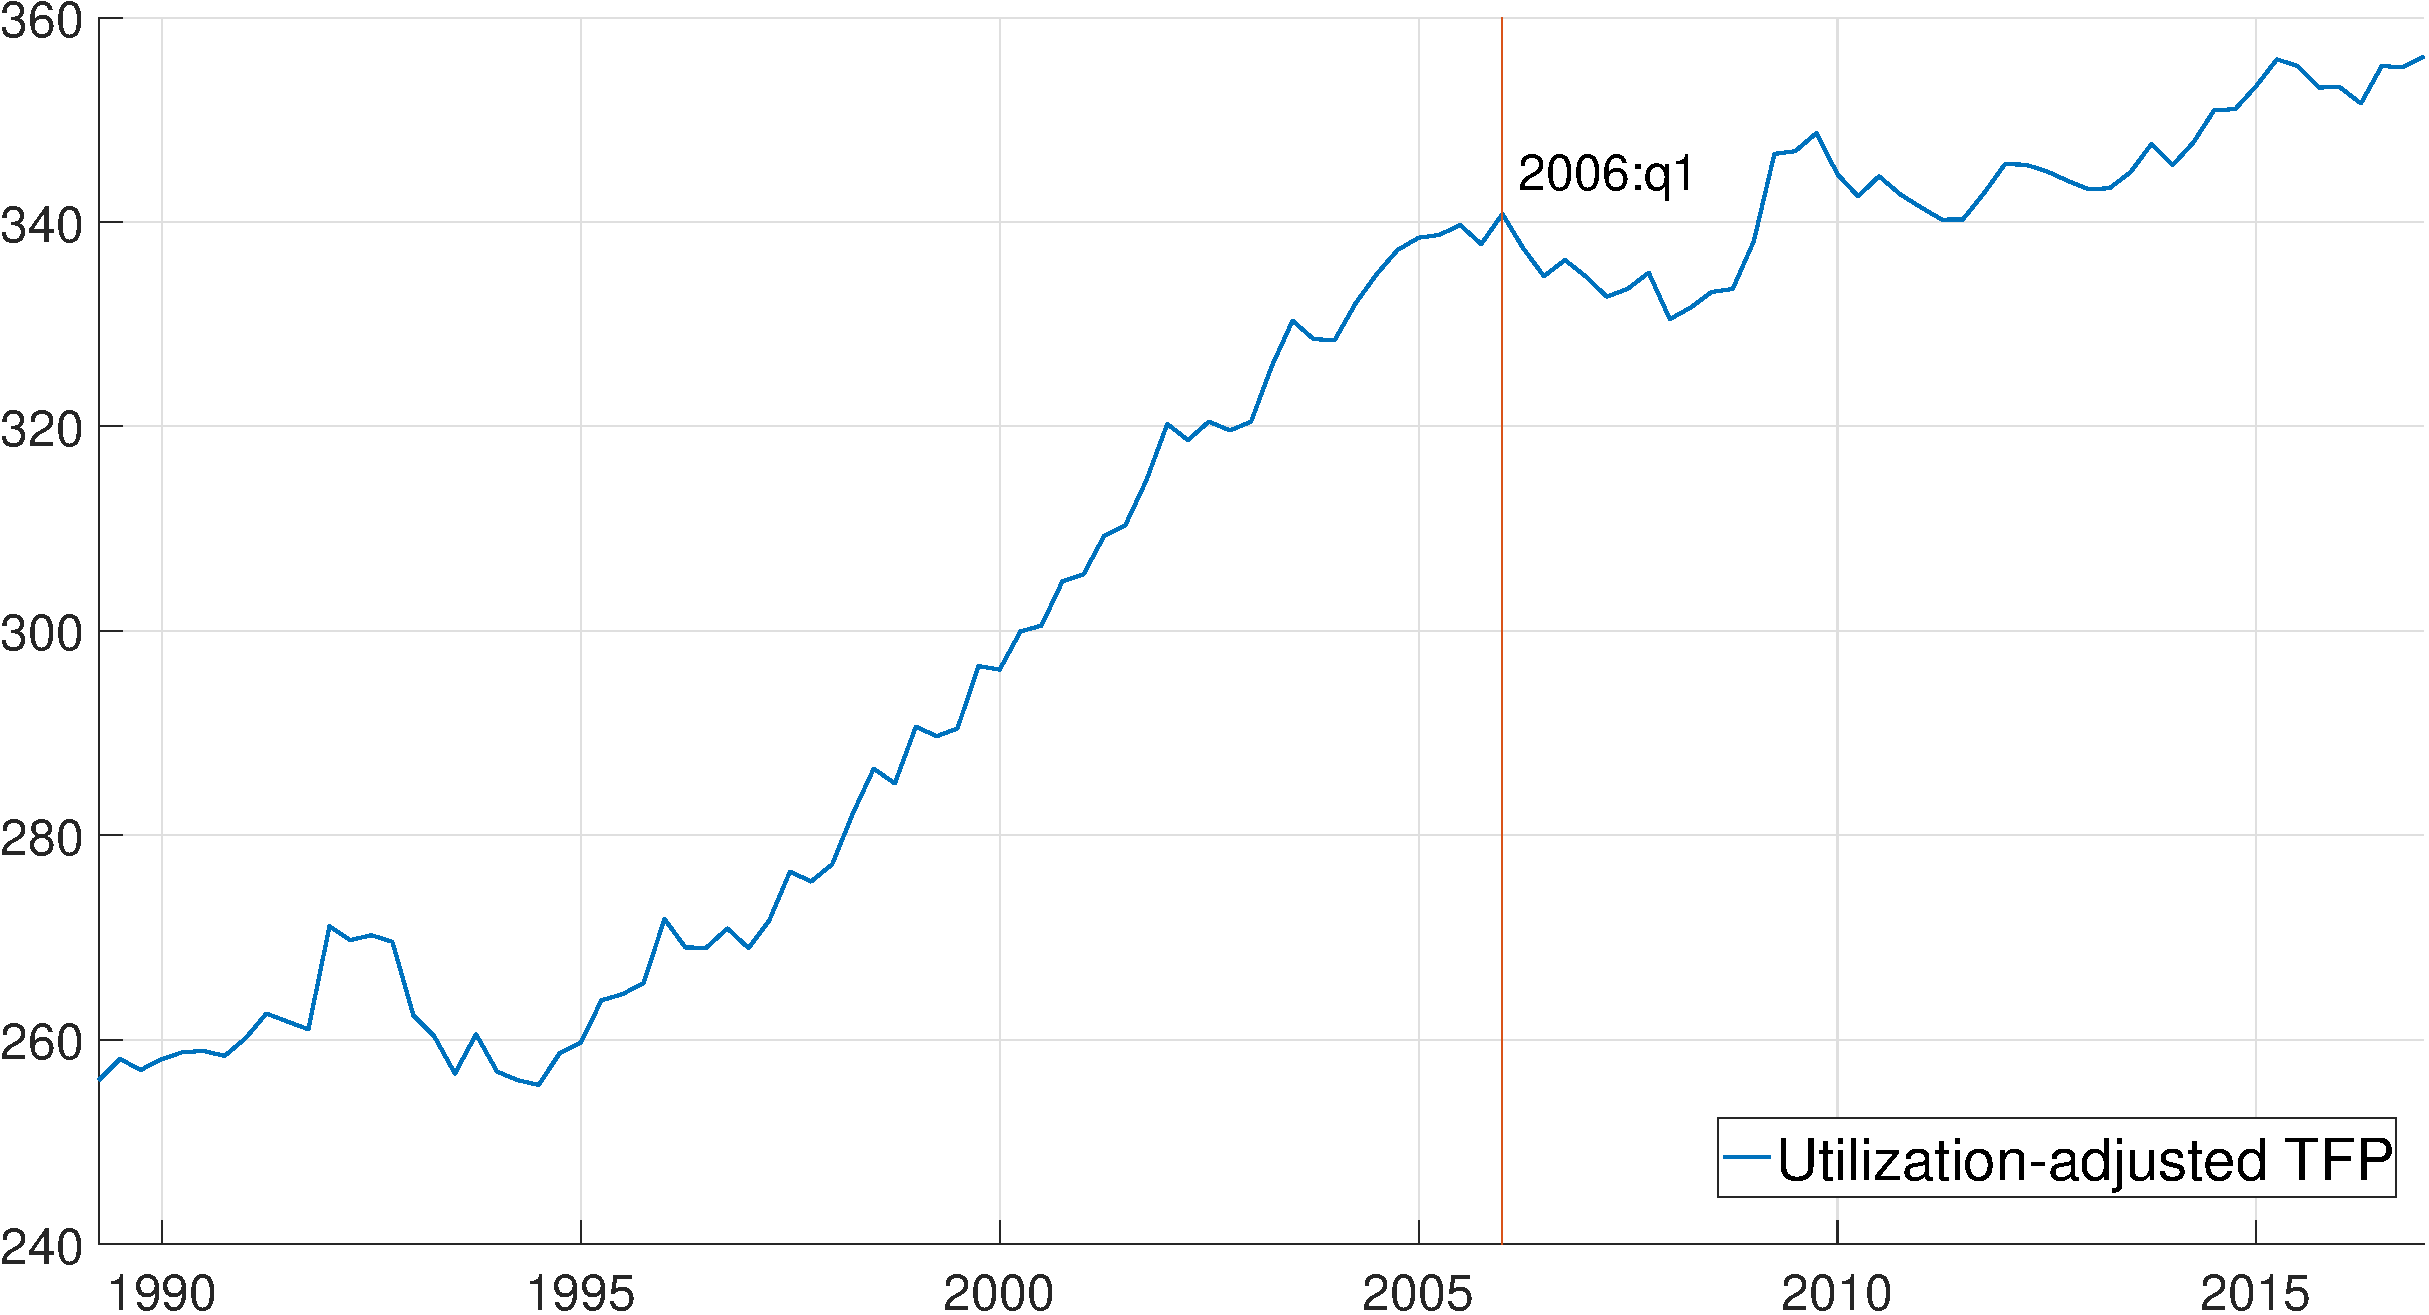
\includegraphics[scale=0.28]{\ourFigPath Figures/fig_TFP_macrolunch_29-Nov-2017_17_41_17}
	\end{figure}
	
	
\end{frame}
%%%%%%%%%%%%%%%%%

%%%%%%% Slide %%%%%%
\begin{frame}
	\frametitle{Two possible mechanisms}
	
\begin{itemize}
\item a permanent, or very persistent exogenous shock to TFP

\

\item an endogenous mechanism
\end{itemize}	

\

\

$\rightarrow$ What we do in a nutshell: test for the endogenous mechanism (main analysis will be a SVAR)


\end{frame}
%%%%%%%%%%%%%%%%%


%%%%%%% Slide %%%%%%
\begin{frame}
	\frametitle{Related literatures}
	\label{related_lit}
\begin{itemize}
\item One strand of literature: Exogenous TFP and news shocks
	\begin{itemize}
	\item Beaudry \& Portier (2006)
	\item Barsky \& Sims (2011)
	
	\end{itemize}
\item [] \textbf{Our contribution: allow in this setting the existence of an endogenous mechanism that affects future TFP}	


\hyperlink{BS_quote}{\beamergotobutton{Barsky \& Sims quote}}

	\
	
	\
	
\item Another strand of literature: Endogenous TFP with R\&D investment as the key variable
	\begin{itemize}
	\item Comin \& Gertler (2006)
	\item Moran \& Queralto (2017)
	
	\end{itemize}	


\item []  \textbf{Our contribution: provide what we think is a more convincing test for the endogenous mechanism}


\end{itemize}



\end{frame}
%%%%%%%%%%%%%%%%%

%%%%%%% Slide %%%%%%
\begin{frame}
	\frametitle{Why more convincing?}
	\label{convincing}
	
	Because the endogenous TFP literature faces a big problem: The endogenous mechanism is rationalized entirely using R\&D investment. 
	
	\
	
\begin{enumerate}
\item  But R\&D in the data is almost acyclical.... $\rightarrow$ hard to rationalize as a driver of business cycle fluctuations % hyperlink to graph: growth rate of RD vs. growth rate of TFP and GDP


\

\item Timing issue: the TFP slowdown begins around 2006, i.e. \emph{before} the Great Recession and thus \emph{before} the marked drop in R\&D  % hyperlink to graph: level of RD and TFP, so we see that TFP drops in 2006, while RD only during the recession.
\hyperlink{timing}{\beamergotobutton{Graph of R\&D}}

\end{enumerate}

\

$\Rightarrow$ Following the suggestion of Fernald, Hall, Stock \& Watson (2009), we propose to use investment in information technology (IT)  % hyperlink to our own graph motivation.pdf: the top graph.
\hyperlink{it_investment}{\beamergotobutton{Graph of IT investment}}

	
	
\end{frame}
%%%%%%%%%%%%%%%%%




%%%%%%% Slide %%%%%%
\begin{frame}
	\frametitle{Empirical analysis}

	We run a SVAR using aggregate, quarterly US data. The data vector is:
	
	\begin{equation}
	\mathbf{X_t} = 
	\begin{bmatrix}
    TFP_t      \\
 
   SP_t   \\
   
   IT_t \\
   
   GDP_t \\
   
   C_t \\
   
   RP_t
\end{bmatrix}
	\end{equation}
	


\

\

\begin{itemize}
\item $RP = \pi^{IT}/\pi^{CPI}$. 
\item All variables are real (except price indexes) and in log levels (except for RP, which is in growth rates). 
\item The dataset ranges from 1989:q1 - 2017:q1.
\end{itemize}	
	
\end{frame}
%%%%%%%%%%%%%%%%%

%%%%%%% Slide %%%%%%
\begin{frame}
	\frametitle{From reduced form to structural form}
	\label{identification}
	
Structural Form	
\begin{equation}
(\mathbf{AD})^{-1}
    \mathbf{X_{t}}
= \mathbf{C(L)} 
\mathbf{X_{t-1}}
+ \mathbf{s_t}
\end{equation}

\

\

Reduced Form
\begin{equation}
\mathbf{X_{t}}
= \underbrace{\mathbf{AD} \mathbf{C(L)}}_\text{$\mathbf{B(L)}$} 
\mathbf{X_{t-1}}
+ \underbrace{\mathbf{AD} \mathbf{_t}}_\text{$\mathbf{i_t}$}
\end{equation}

\

\

\begin{itemize}
	\item $AD$ is the impact matrix
	\item $A$ is s.t. $As_t s_t' A' = i_t i_t' = \Sigma$ and $s_t s_t' = I$
	\item $D$ is a rotation matrix s.t. $DD' = I$ $\Rightarrow$ $AD(AD)' = \Sigma$
\end{itemize}

$D$ will be a tool to impose our identification assumptions \hyperlink{Technicalities}{\beamergotobutton{Technicalities}}

\end{frame}
%%%%%%%%%%%%%%%%%

%%%%%%% Slide %%%%%%
\begin{frame}
\frametitle{Identified shocks}


\begin{itemize}
	\item We impose restrictions on $D$ in order to identify two shocks:
	\begin{enumerate}
		\item News Shock
		\item IT Productivity Shock
	\end{enumerate}

\
	
	\item Econometric challenge is to disentangle two shocks with very similar features 
		\begin{enumerate}
		\item No impact effect on TFP
		\item Persistent positive effect over time on TFP
		\item Most likely both shocks have positive impact effects on forward-looking variables
	\end{enumerate}

\
	
	
	\item Barsky \& Sims' identification strategy is not sufficient to disentangle the two
	\begin{itemize}
		\item We need a further assumption (restriction) to find a dimension of difference between the shocks
	\end{itemize}
\end{itemize}


\end{frame}
%%%%%%%%%%%%%%%%%

%%%%%%% Slide %%%%%%
\begin{frame}
\frametitle{Additional restriction}


\begin{itemize}
	\item We rely on simple demand and supply theory
	
	\
	
	\begin{enumerate}
		\item The IT shock is a \emph{sectoral} shock $\rightarrow$ we expect it to move relative prices
		\item The news shock is \emph{not} a sectoral shock $\rightarrow$ we have no a priori sense of what it should do to relative prices on impact, but after some time relative prices should go back to their initial value
	\end{enumerate}
	
	\
	
\end{itemize}

	$\rightarrow$ add the restriction that a news shock should have no effect on relative prices after a reasonable time
	
\hspace{4cm} $\hookrightarrow$ enough for prices to adjust, so

\hspace{4cm}   between 6-12 quarters 


\end{frame}
%%%%%%%%%%%%%%%%%

%%%%%%% Slide %%%%%%
\begin{frame}
	\frametitle{Identification strategy overall}

\begin{equation}
TFP_t =  \underbrace{\varepsilon_t}_\text{surprise tech shock}  + \underbrace{V_{t-k}}_\text{news shock} + \underbrace{IT_{t-k}}_\text{IT shock}  
\end{equation}

\

    \begin{enumerate}
    	\item The news shock $V_{t-k}$ maximizes the FEV of future TFP subject to the restriction that it has no effect on the relative price $RP$ at a small number of quarters;
	
	\
	
    \item The IT shock maximizes the remaining FEV of future TFP;
    
    \
    
    \item The tech shock $\varepsilon_t$ is considered as a residual shock and is left unrestricted (unidentified).
   \end{enumerate}
	
	
\end{frame}
%%%%%%%%%%%%%%%%%

%%%%%%% Slide %%%%%%
\begin{frame}
	\frametitle{Our favorite specification}
	
	\begin{itemize}
	\item Recall: dataset is quarterly and covers 1989:q1-2017-q1.
	
	\
	
	\item One lag (as suggested by BIC and HQ).
	
	\
	
	\item Horizon of FEV-maximization: 100 quarters.
	
	\
	
	\item Restriction on relative prices after a news shock is imposed at 8 quarters.
	
	\end{itemize}


	
	
\end{frame}
%%%%%%%%%%%%%%%%%

%%%%%%%%%%%%%%%%%%%%%%%%%
\begin{frame}
\frametitle{TFP response to both shocks}
\begin{figure}
	\centering
	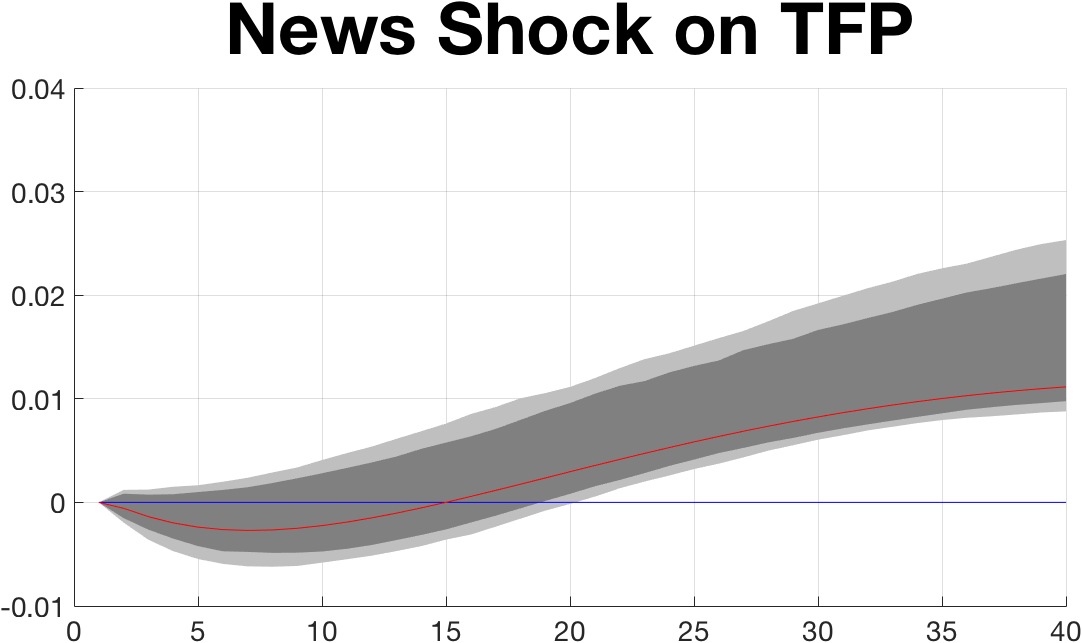
\includegraphics[scale=0.15]{\ourFigPath Figures/fig_News_Shock_on_TFP__}
\end{figure}
\begin{figure}
	\centering
	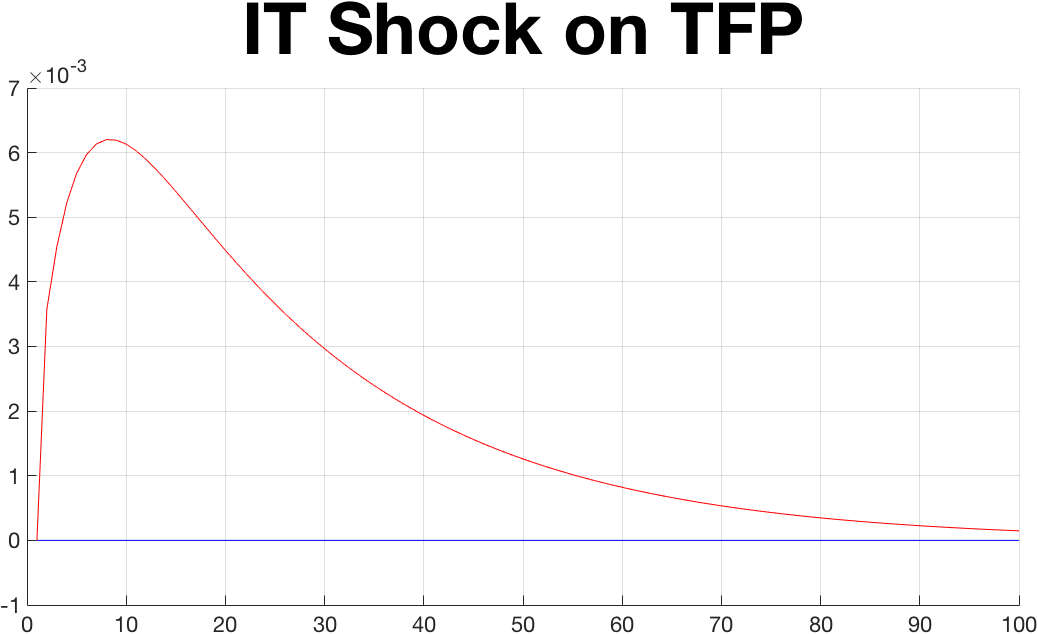
\includegraphics[scale=0.15]{\ourFigPath Figures/fig_IT_Shock_on_TFP__}
\end{figure}
\end{frame}
%%%%%%%%%%%%%%%%%%%%%%%%%%%%%

%%%%%%%%%%%%%%%%%%%%%%%%%
\begin{frame}
\frametitle{Real SP500 response to both shocks}
\begin{figure}
	\centering
	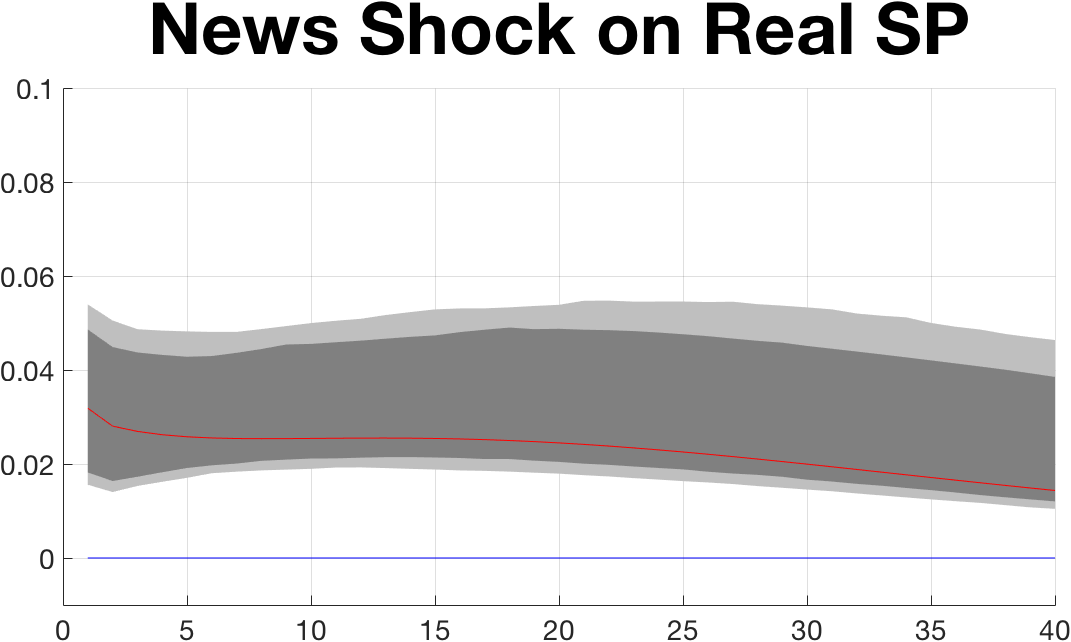
\includegraphics[scale=0.15]{\ourFigPath Figures/fig_News_Shock_on_Real_SP__}
\end{figure}
\begin{figure}
	\centering
	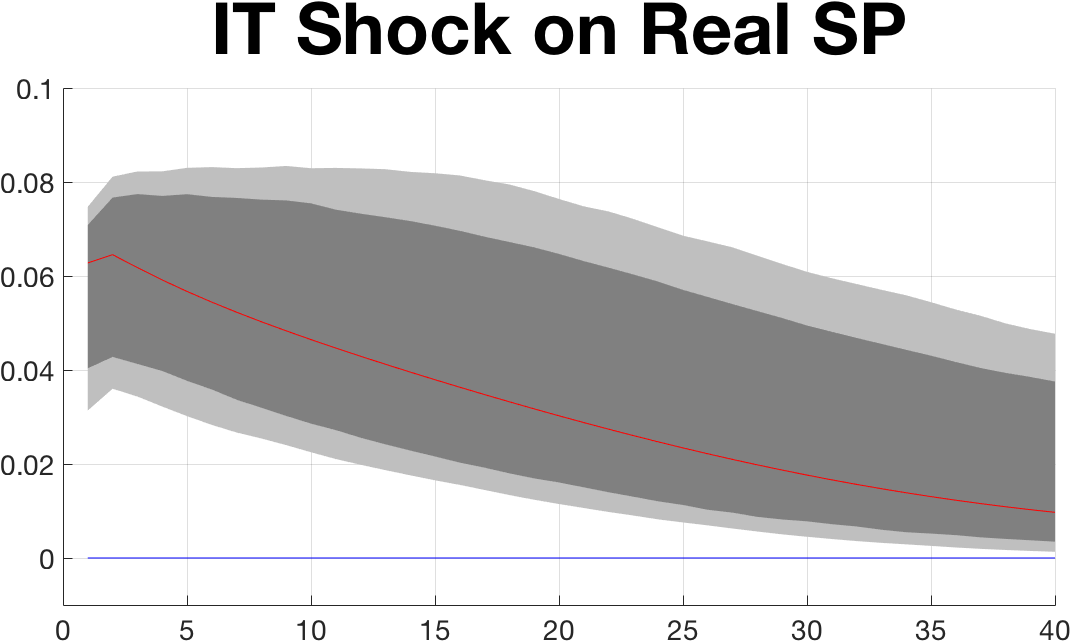
\includegraphics[scale=0.15]{\ourFigPath Figures/fig_IT_Shock_on_Real_SP__}
\end{figure}
\end{frame}
%%%%%%%%%%%%%%%%%%%%%%%%%%%%%

%%%%%%%%%%%%%%%%%%%%%%%%%
\begin{frame}
\frametitle{IT investment response to both shocks}
\begin{figure}
	\centering
	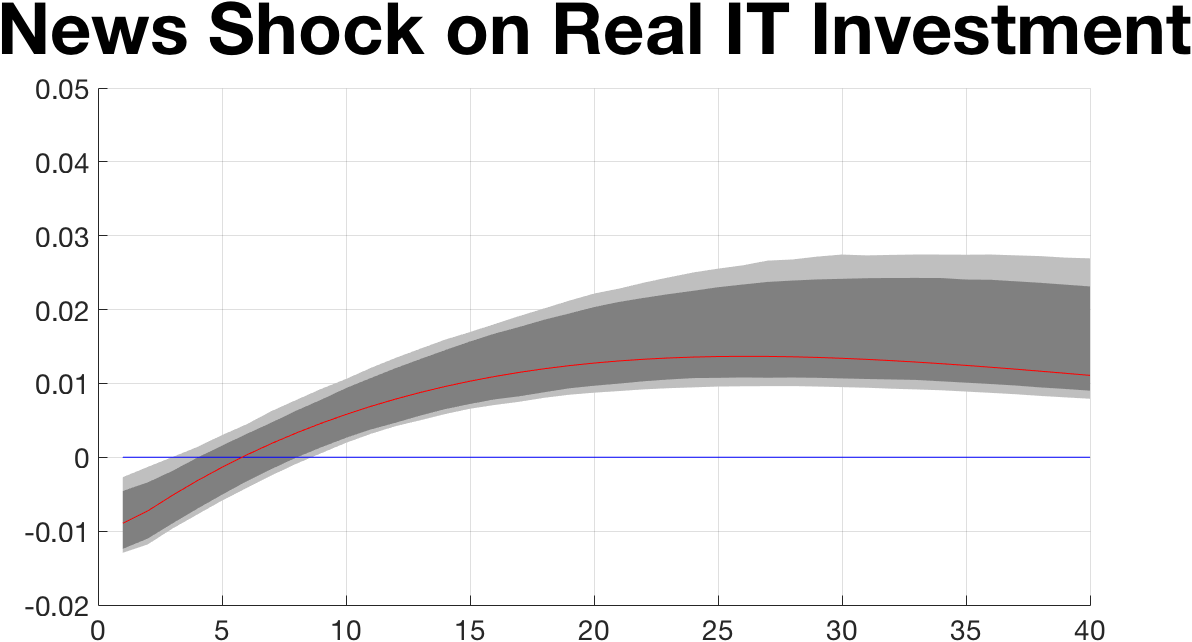
\includegraphics[scale=0.15]{\ourFigPath Figures/fig_News_Shock_on_Real_IT_Investment__}
\end{figure}
\begin{figure}
	\centering
	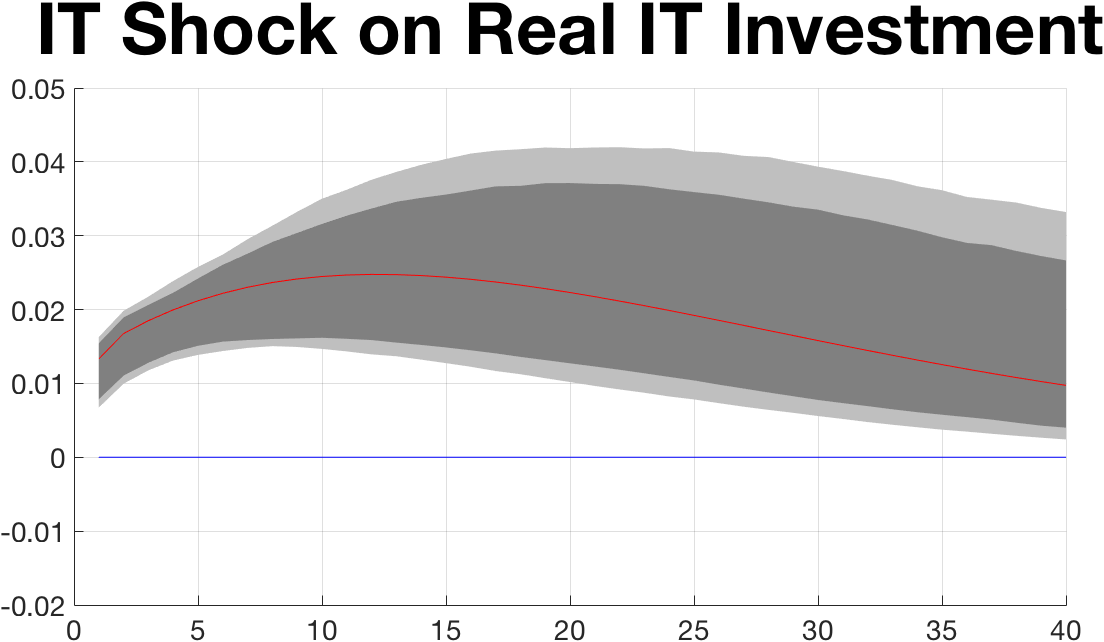
\includegraphics[scale=0.15]{\ourFigPath Figures/fig_IT_Shock_on_Real_IT_Investment__}
\end{figure}
\end{frame}
%%%%%%%%%%%%%%%%%%%%%%%%%%%%%


%%%%%%%%%%%%%%%%%%%%%%%%%
\begin{frame}
\frametitle{Other responses to  both shocks}

\vspace{-0.2cm}
\begin{figure}
\begin{multicols}{2}
\centering 
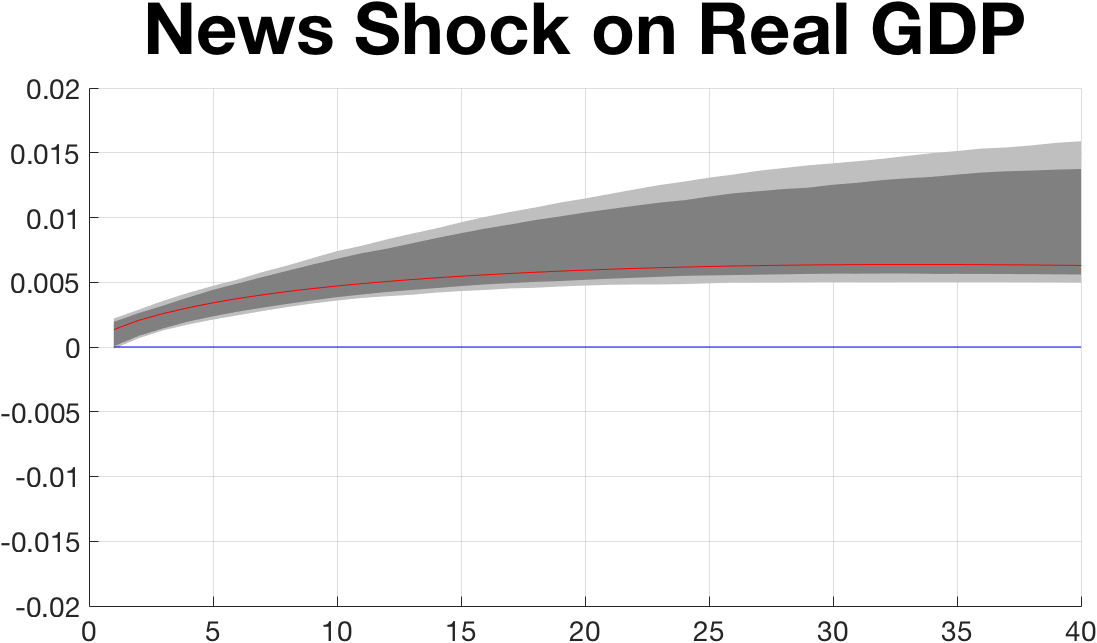
\includegraphics[scale = 0.1]{\ourFigPath Figures/fig_News_Shock_on_Real_GDP_Ryan_two_stepsID_10-Dec-2017_17_34_47}\\ 
\vspace{0.3cm}
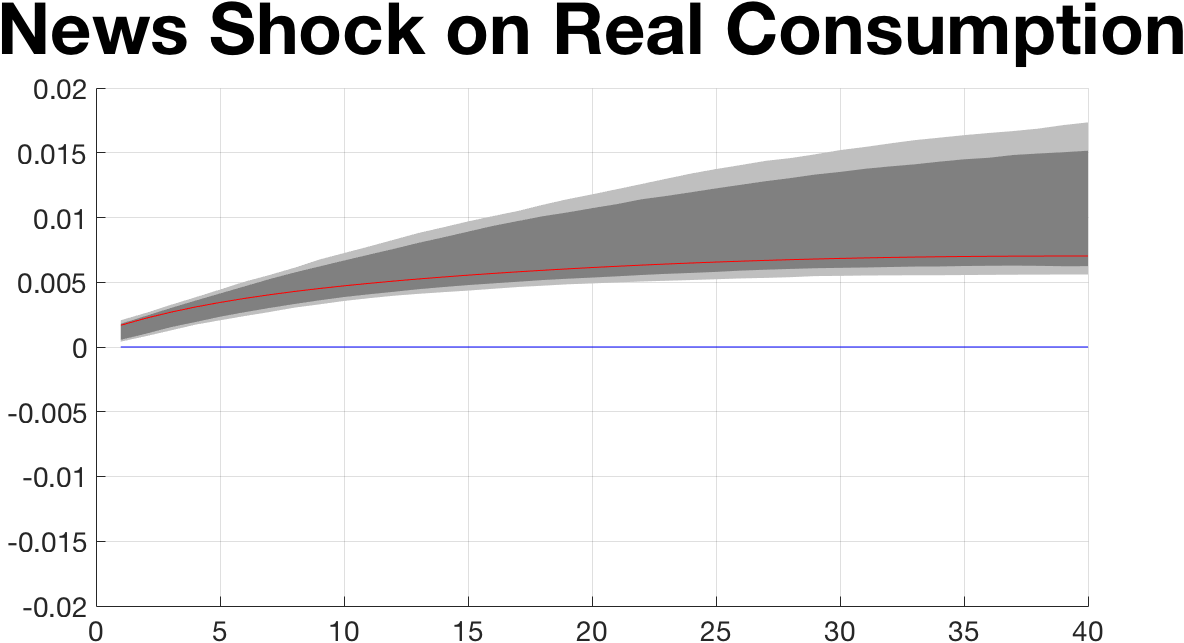
\includegraphics[scale = 0.1]{\ourFigPath Figures/fig_News_Shock_on_Real_Consumption_Ryan_two_stepsID_10-Dec-2017_17_34_50}\\ 
\vspace{0.3cm}
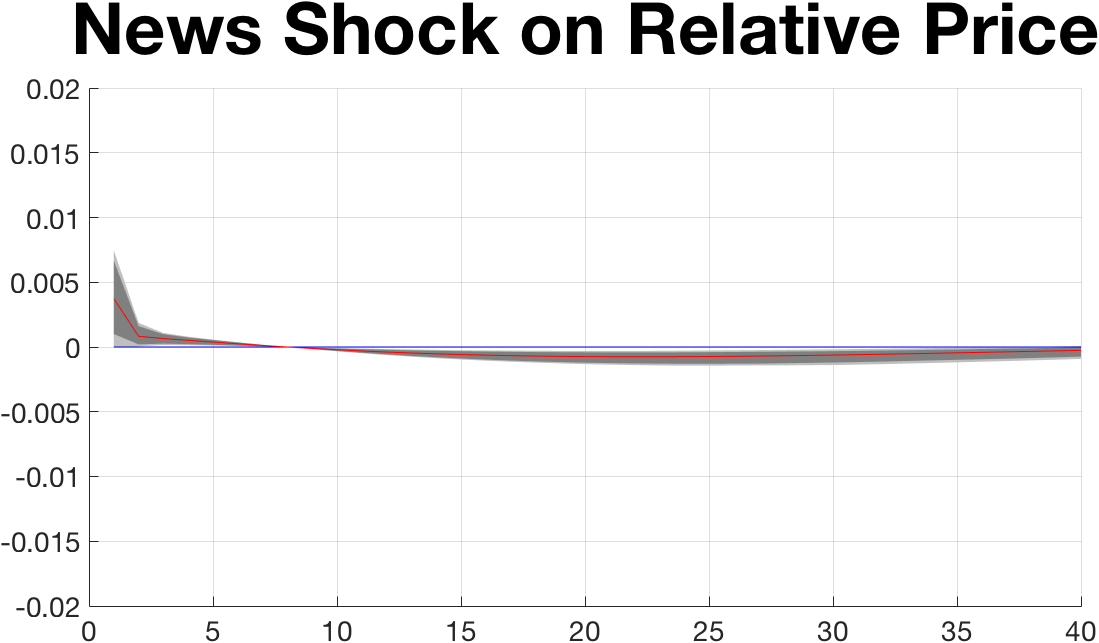
\includegraphics[scale = 0.1]{\ourFigPath Figures/fig_News_Shock_on_Relative_Price_Ryan_two_stepsID_10-Dec-2017_17_34_52}\\ 


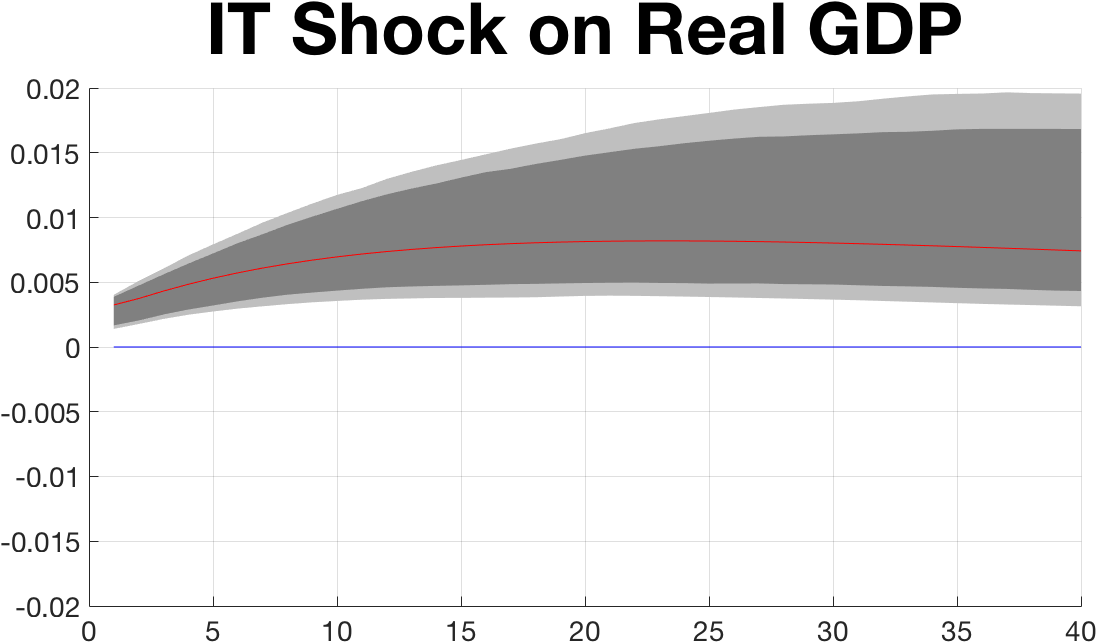
\includegraphics[scale = 0.1]{\ourFigPath Figures/fig_IT_Shock_on_Real_GDP_Ryan_two_stepsID_10-Dec-2017_17_35_00}\\
\vspace{0.3cm}
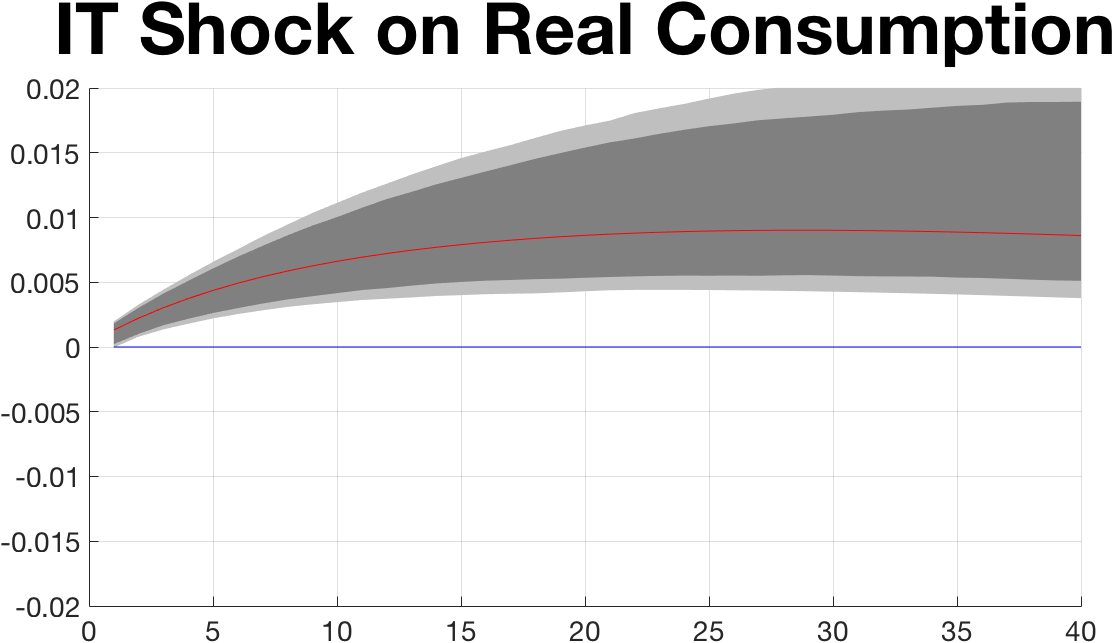
\includegraphics[scale = 0.1]{\ourFigPath Figures/fig_IT_Shock_on_Real_Consumption_Ryan_two_stepsID_10-Dec-2017_17_35_02}\\ 
\vspace{0.3cm}
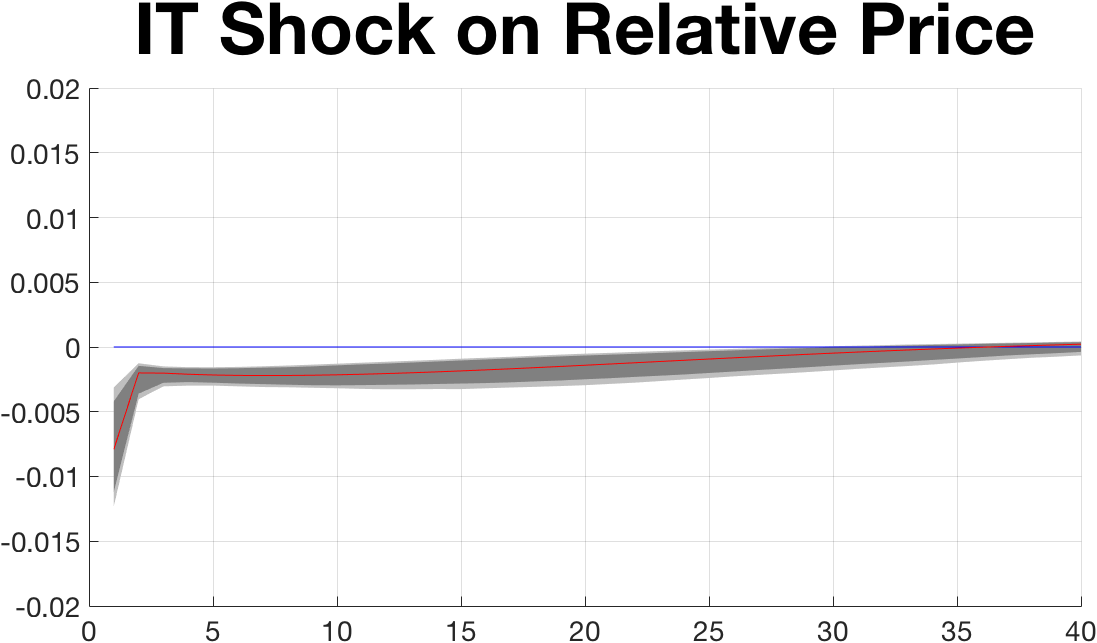
\includegraphics[scale = 0.1]{\ourFigPath Figures/fig_IT_Shock_on_Relative_Price_Ryan_two_stepsID_10-Dec-2017_17_35_04}\\ 

\end{multicols}
\end{figure}


\end{frame}
%%%%%%%%%%%%%%%%%%%%%%%%%%%%%


%%%%%%% Slide %%%%%%
\begin{frame}
	\frametitle{FEV explained by the two shocks at 40 periods}


    \hspace{2.25cm}
\begin{large}
	\begin{tabular}{lccc}
	\hline
		& News & IT & Total \\
		\hline
	TFP	           & 0.20384  & 0.52596 & 0.72981  \\
		\hline
	\end{tabular}
\end{large}
		 	
\end{frame}
%%%%%%%%%%%%%%%%%

%%%%%%% Slide %%%%%%
\begin{frame}
	\frametitle{Interpretation}

\begin{enumerate}
 \item Shape and timing of the responses reflect ...
 
 %\ 
 
	\begin{itemize}
	\item both the Barsky \& Sims result ...
	
	\vspace{0.1cm}
	
	\item ... as well as the the conjecture that the IT shock looks similar to news along certain dimensions, 
	
	\vspace{0.1cm}
	
	\item ... but relative prices do indeed introduce a margin of difference between the two shocks.
	\end{itemize}

\

\item Shares of FEV of TFP explained ...
	\begin{itemize}
	\item ... are also in line with the Barsky \& Sims result ...
	\item [] For BS, news explains around 45\%, compared to 20\% here
	
	\vspace{0.1cm}
	
	\item ... yet suggest that the IT shock plays an important role as well (around 52\%)
	
	\vspace{0.1cm}
	
	\item ... and indeed the IT shock \emph{complements} the news shock, instead of substituting for it
	\item [] For BS, the single identified shock explains around 45\%, while our two identified shocks explain around 73\%
	\end{itemize}

\end{enumerate}
		 	
\end{frame}
%%%%%%%%%%%%%%%%%

%%%%%%% Slide %%%%%%
\begin{frame}
	\frametitle{Robustness checks}

\begin{itemize}
\item Different variables
	\begin{itemize}
	\item Add the Michigan index of consumer confidence (expected business conditions 5 years ahead)
	
	
	\
	
	\item Replace IT prices with capital prices (following Comin \& Gertler)
	\end{itemize}
	
	\
	
\item Different horizons at which we impose the restriction on relative prices for the news shock
\item[] $\rightarrow$ ran  6, 8, 10, 12 and 16 quarters.

\

\item Increase the number of lags (2)

\

\item Check whether VAR is information-sufficient to identify the news shock (Forni-Gambetti test) (p-val of 12\%)
\end{itemize}
   		 	
\end{frame}
%%%%%%%%%%%%%%%%%

%%%%%%% Slide %%%%%%
\begin{frame}
	\frametitle{Conclusion}
	
\begin{itemize}
\item Provided what we think (and we hope you do too) a careful and more general test for the endogenous mechanism in TFP.
\begin{itemize}
\item While the literature focuses exclusively on R\&D, we show that IT is a better variable to focus on.
\end{itemize}

\ 

\item The results show that by controlling for the presence of news shocks, the endogenous component of TFP is an important driver of TFP fluctuations at long horizons.

\

\item This result does not contrast however with the findings of the news shock literature since we still find that news also play a significant role in explaining TFP.

\end{itemize}
   		 	
\end{frame}
%%%%%%%%%%%%%%%%%

%%%%%%% Slide %%%%%%
\begin{frame}
	\frametitle{Work ahead}
	
\begin{itemize}
\item Rationalize this setting using a theoretical model
\item [] $\hookrightarrow$ what we have in mind: an endogenous TFP model (in the vein of Comin \& Gertler) augmented with news shocks 

\

\item Estimate the model (IR-matching)

\

\item Perform a counterfactual for the Great Recession \emph{and} the period prior, shutting down the negative IT shocks around 2000
% assuming the IT bubble, i.e. the negative shock to IT productivity around 2000, did not happen.

\

\item See if we can find interesting interactions between the two shocks?
\item [] $\hookrightarrow$ In particular, we're thinking of noise shocks on IT productivity
	\begin{itemize}
	\item [] news shock: shock to expected future value
	\item [] noise shock: shock to expected current value (``perceptions'')
	\end{itemize}
\end{itemize}


   		 	
\end{frame}
%%%%%%%%%%%%%%%%%





%%%%%%%%%%%%%%%%%%%%%%%%%%%%%%%%%%%%%%%%%%%%%%%%%%%%%%%%%%%%%%%%%%%%%%
%%%%%%                     APPENDIX  
%%%%%%%%%%%%%%%%%%%%%%%%%%%%%%%%%%%%%%%%%%%%%%%%%%%%%%%%%%%%%%%%%%%%%%


%%%%%%% Slide %%%%%%
\begin{frame}
	\frametitle{Barsky \& Sims say:}
	\label{BS_quote}
	
\blockquote{\emph{A more general objection to our empirical approach would be that a number of structural shocks, which are not really ``news'' in the sense defined by the literature, might affect a measure of TFP in the future without impacting it immediately. Among these shocks might be research and development shocks, investment specific shocks, and reallocative shocks. Our identification (and any other existing VAR identifications) would obviously confound any true news shock with these shocks.}}

\

\hspace{5cm} Barsky \& Sims (2011), p. 278.

\

\

\
	
\hyperlink{related_lit}{\beamerreturnbutton{Return}}	
\hyperlink{BS_FEV}{\beamerbutton{Barsky \& Sims' FEV-table}}	
\end{frame}
%%%%%%%%%%%%%%%%%

%%%%%%% Slide %%%%%%
\begin{frame}
	\frametitle{Barsky \& Sims FEV of TFP explained}
	\label{BS_FEV}
	

\vspace{-1cm}
\noindent
\begin{figure}
\centering
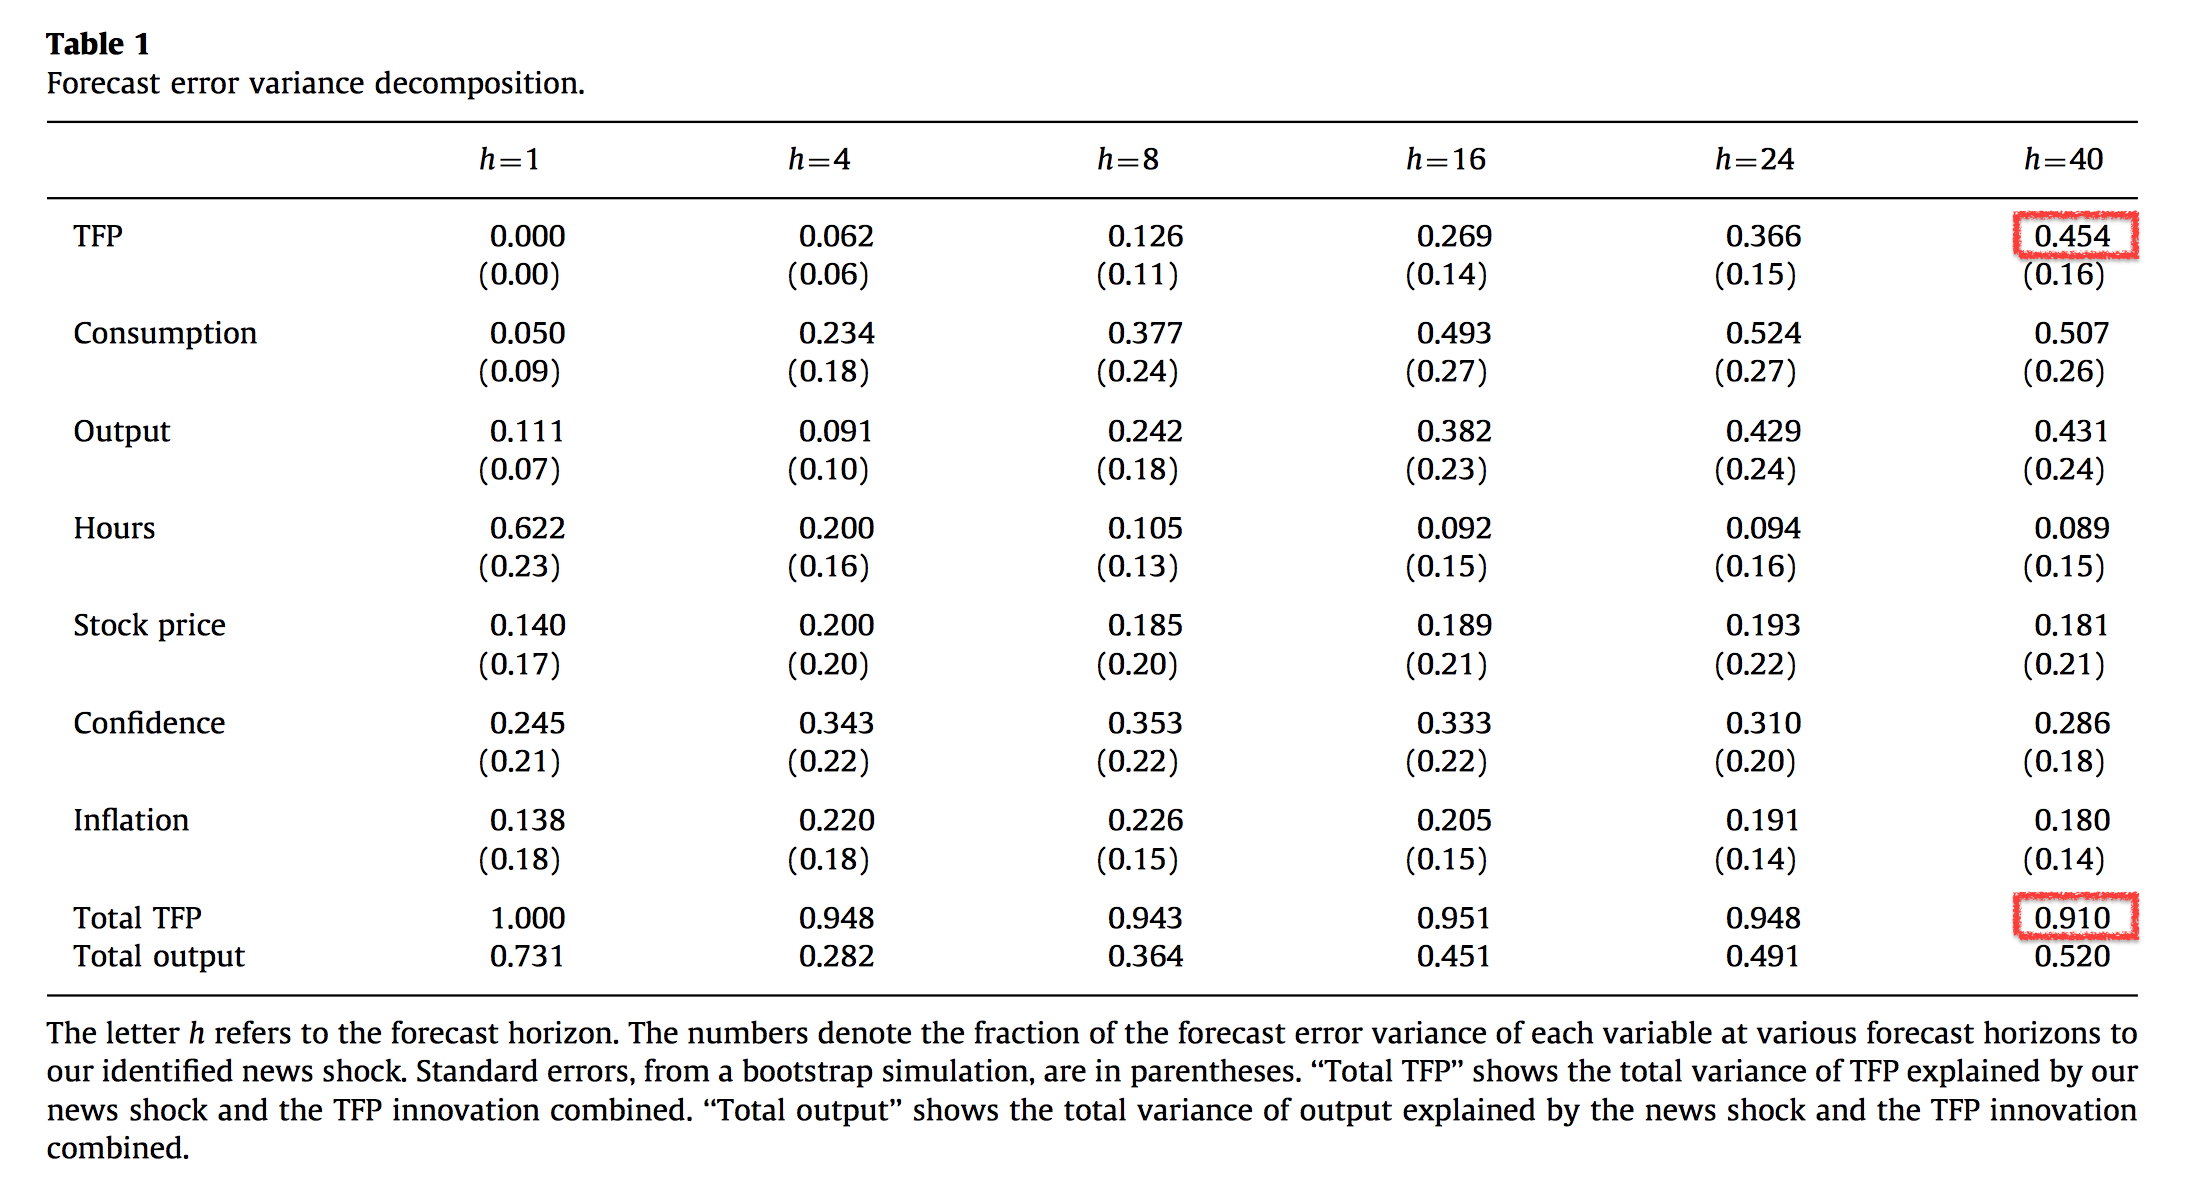
\includegraphics[scale=0.3]{fig_BS_fevtable}
\end{figure}
	
\hyperlink{related_lit}{\beamerreturnbutton{Return}}	
\end{frame}
%%%%%%%%%%%%%%%%%


%%%%%%% Slide %%%%%%
\begin{frame}
	\frametitle{Timing: RD drop vs TFP drop}
	\label{timing}
	
	\vspace{-1cm}
	\noindent
	\begin{figure}
		\centering
		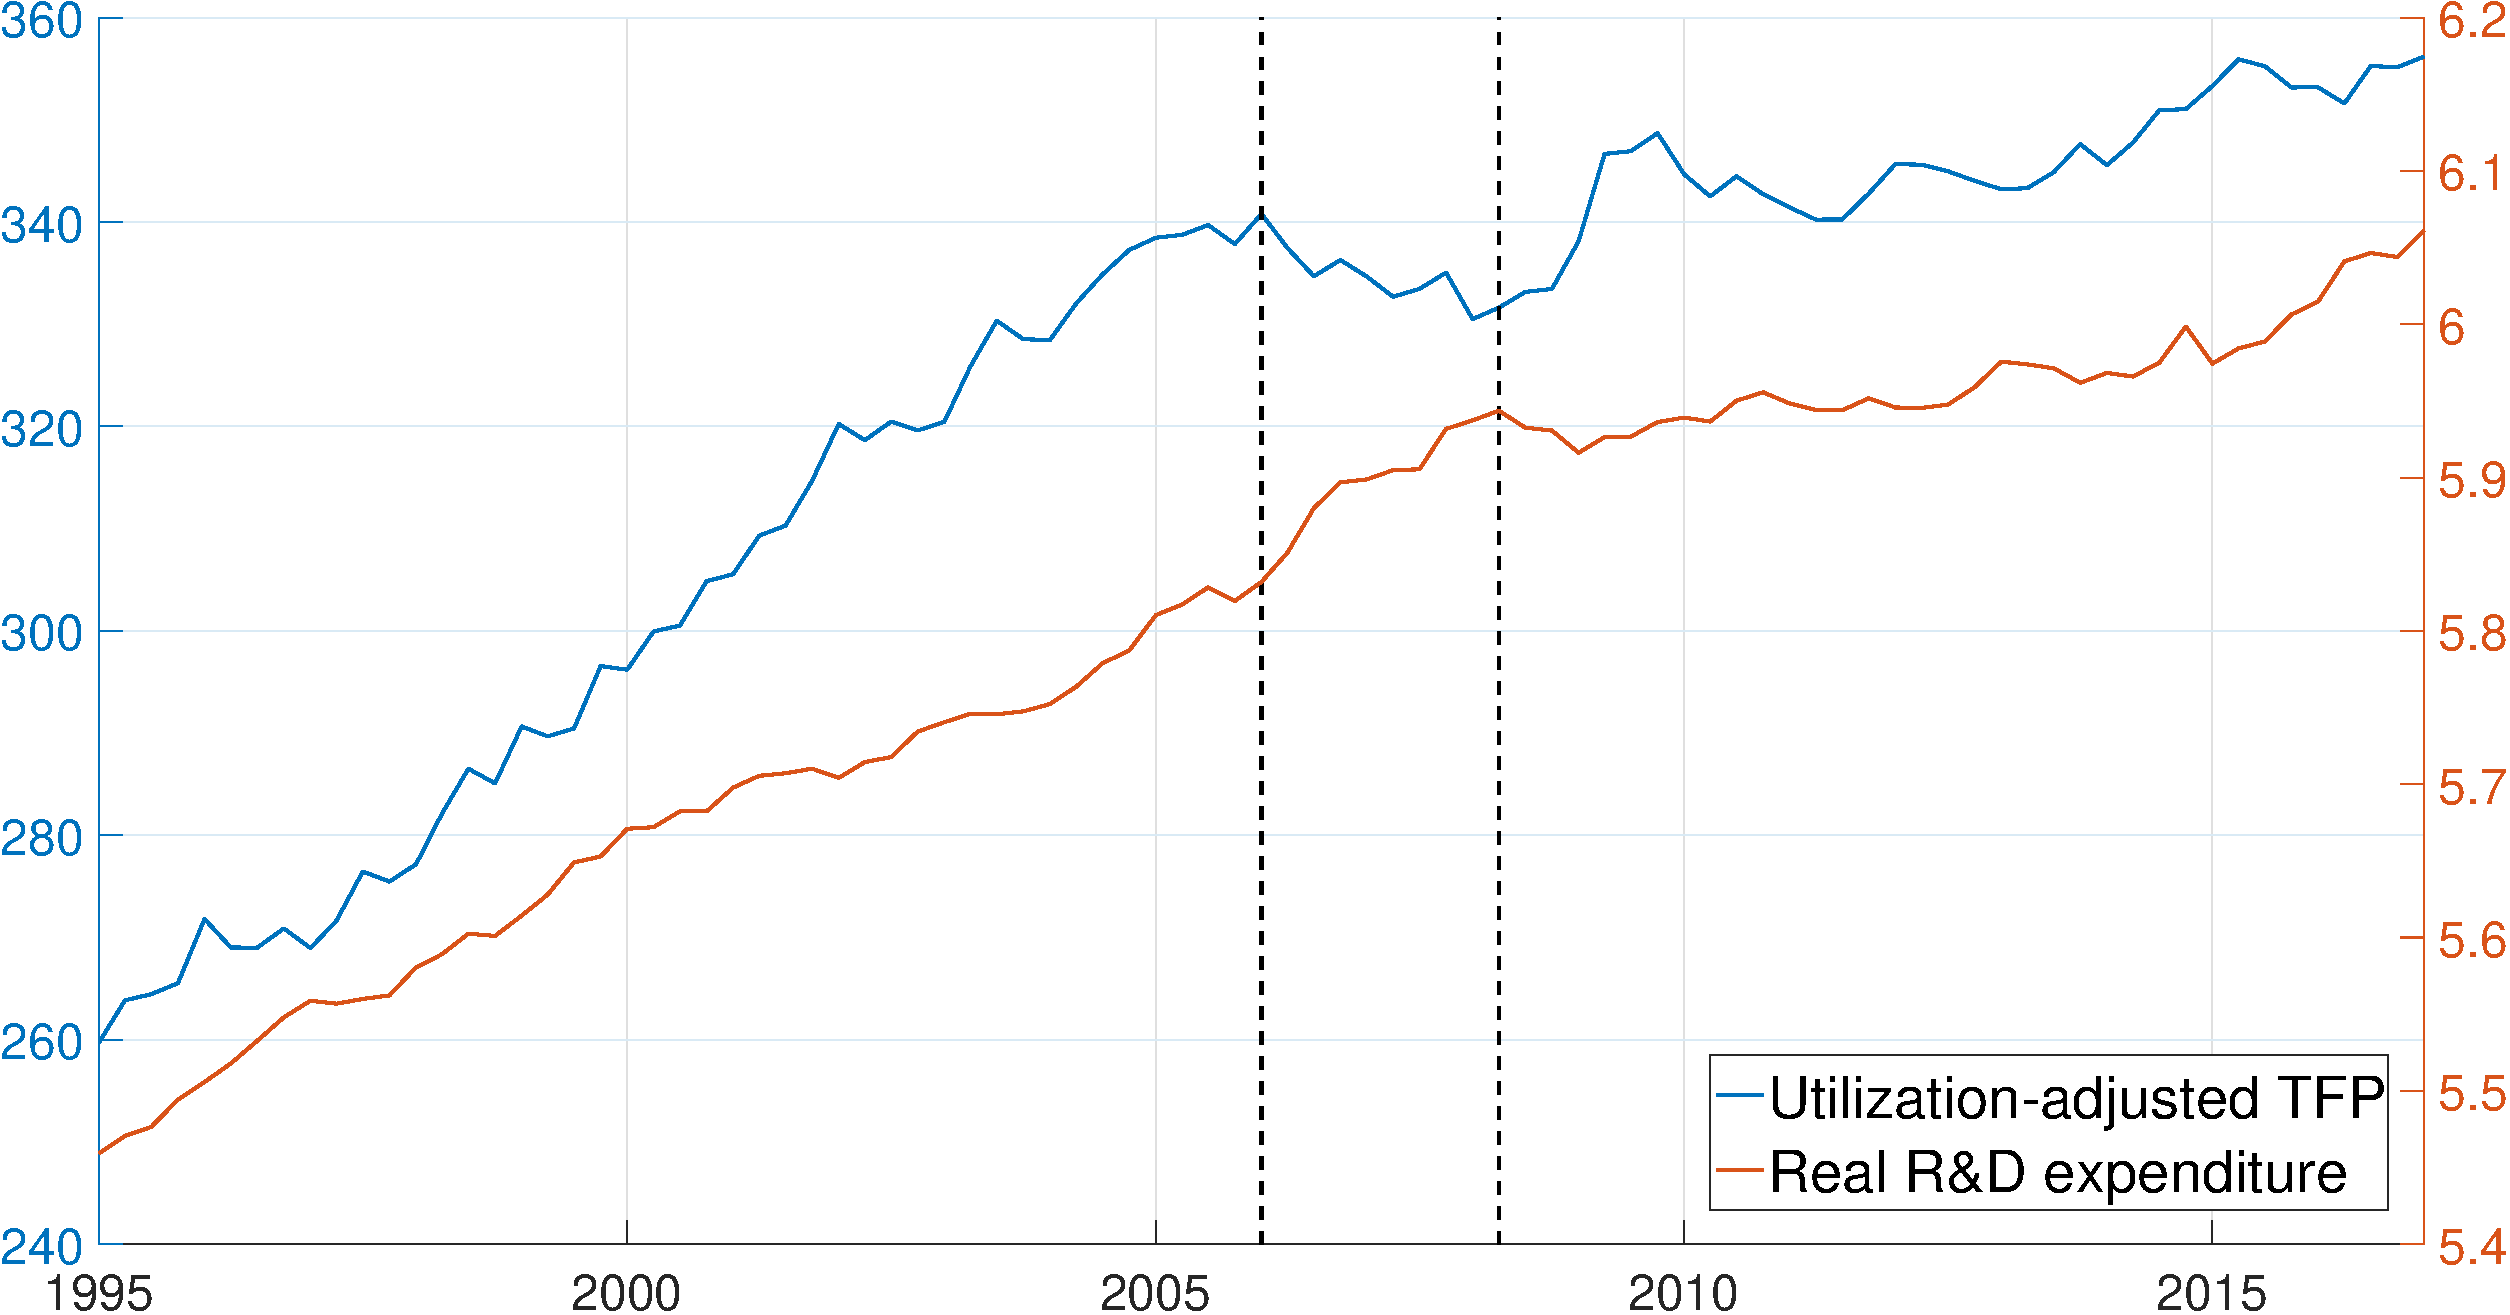
\includegraphics[scale=0.28]{\ourFigPath Figures/fig_RD_level_macrolunch_30-Nov-2017_11_31_04}
	\end{figure}

	
\hyperlink{convincing}{\beamerreturnbutton{Return}}	
\end{frame}
%%%%%%%%%%%%%%%%%

%%%%%%% Slide %%%%%%
\begin{frame}
	\frametitle{IT investment: a drop at the right time}
	\label{it_investment}
	
%	\vspace{-1cm}
	\noindent
	\begin{figure}
		\centering
		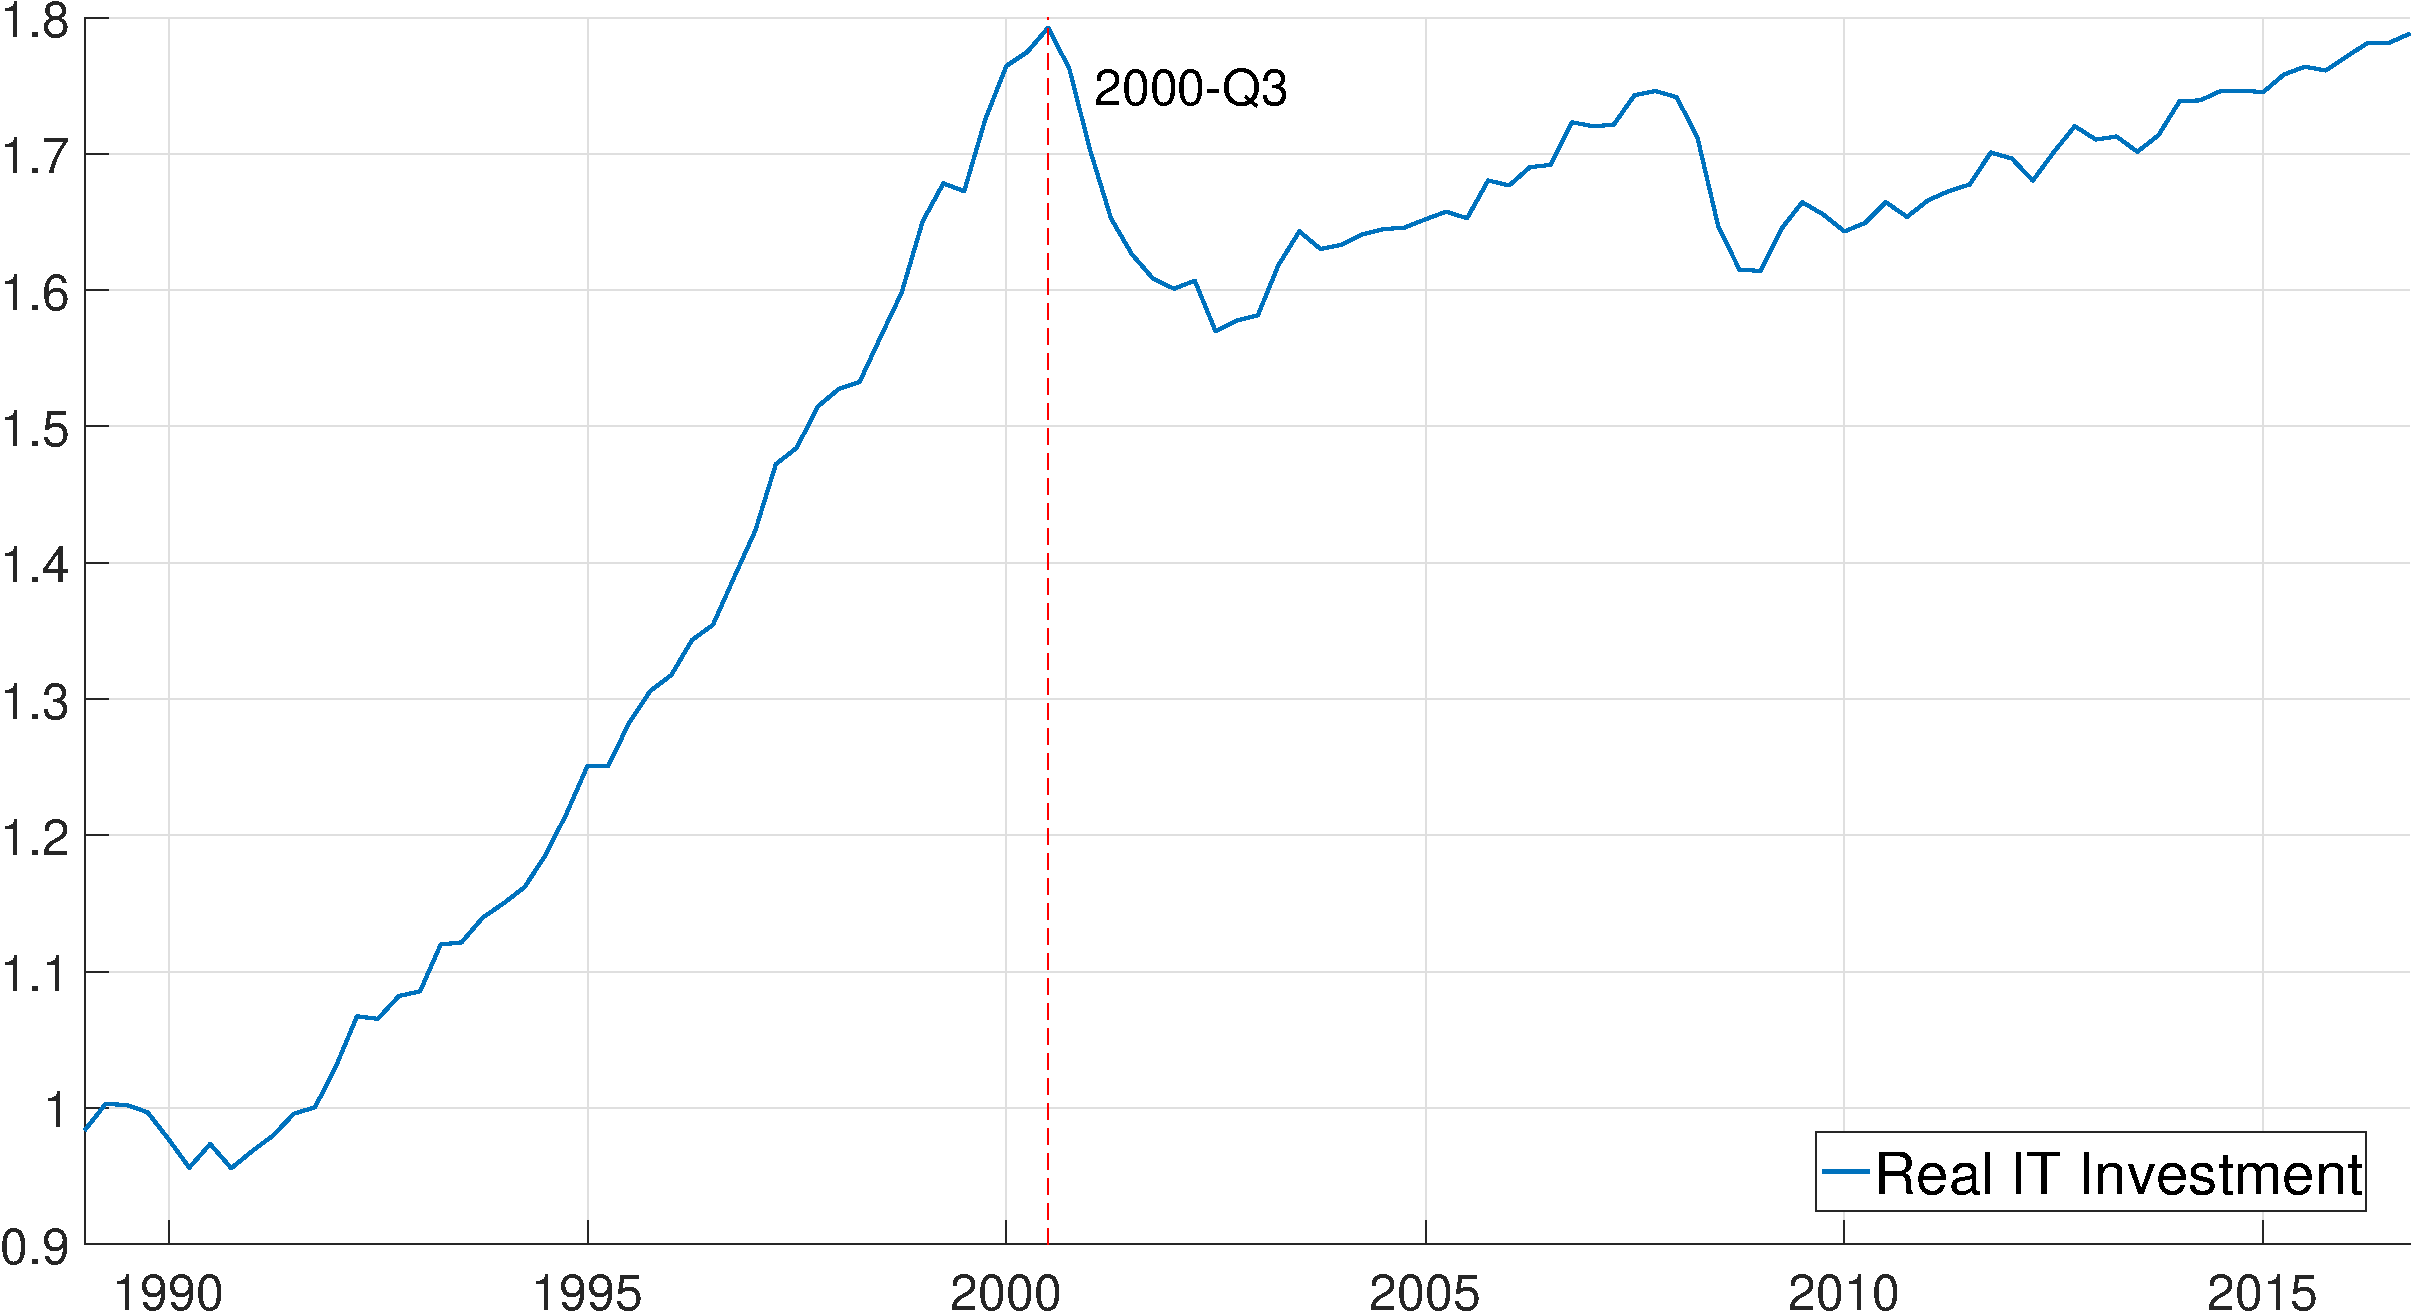
\includegraphics[scale=0.29]{\ourFigPath Figures/fig_IT_level_macrolunch_30-Nov-2017_11_37_26}
	\end{figure}

	
\hyperlink{convincing}{\beamerreturnbutton{Return}}	
\end{frame}
%%%%%%%%%%%%%%%%%

%%%%%%% Slide %%%%%%
\begin{frame}
\frametitle{Identification Strategy}
\label{Technicalities}

\begin{equation}
D = \begin{bmatrix}
d_{11} & \gamma_{12} & \gamma_{13} & d_{14} & \cdots \\
d_{21} & \gamma_{22} & \gamma_{23} & d_{24} & \cdots \\
\vdots & \vdots & \vdots & \ddots & \vdots 
\end{bmatrix}
\end{equation}

\begin{itemize}
	\item Indifferent over $d_{ij}$ as long as $D$ is orthogonal
	\item $A \gamma_{2}$ is the impact response to a news shock
	\item $A \gamma_{3}$ is the impact response to a IT productivity shock
	\item First element of both $A \gamma_{2}$ and $A \gamma_{3}$ is zero due to the no-contemporaneous effect of both shocks on TFP
	\item $A \gamma_2$ is such that the FEV of TFP is maximized subject to zero long-run effect on $RP$
	\item $A \gamma_3$ is maximizing the remaining FEV of TFP 
\end{itemize} 


\hyperlink{identification}{\beamerreturnbutton{Return}}	
\end{frame}
%%%%%%%%%%%%%%%%%
	
	





















\end{document}
